\section{Music Structure Analysis as downstream task}

While the usefulness of deep audio embeddings can be evaluated in countless downstream tasks, we have chosen Music Structure Analysis (MSA) for its popularity, complexity, and product-compelling nature. This interdisciplinary field aims to understand the structure of music \cite{Nieto2020Audio-BasedApplications}. Due to subjectivity, ambiguity, and data scarcity, audio-based MSA faces challenges like boundary placement ambiguity and similarity quantification \cite{NietoPerceptualMusic}. 

The main principles of MSA were initially defined as homogeneity, novelty, and repetition, with the addition of regularity. 

\subsection{SALAMI dataset}

SALAMI (Structural Analysis of Large Amounts of Music Information) aims to conduct massive structural analyses of different types of music \cite{Smith2011DESIGNANNOTATIONS}. The project covers diverse music, from Western pop to Indian classical and from live to studio recordings.

The authors propose a unique music analysis approach that segments pieces into sections rather than traditional forms. Their method combines perceptual, functional, and transcription analyses, considers music's hierarchical nature, and uses markers to determine analysis timescales. While providing a comprehensive investigation, each analysis approach has limitations in accurately reflecting musical structure, labeling identical or different music sections, and capturing the complete structural framework. This innovative approach aims for a more nuanced, holistic music analysis.

\section{\textit{Embeddiogram} feature}

The \textit{embeddiogram} is derived by applying our pre-trained neural network model to sliding windowed segments across the audio signal, generating a sequence of embedding vectors. These relatively high-dimensional embedding vectors collectively form a two-dimensional description of the audio signal's musical content.

Below is a detailed explanation of how we compute the \textit{embeddiogram} from a given audio signal. This process comprises five key steps, including loading the audio data, slicing the audio data into windowed segments, processing each window using a pre-trained model to produce an embedding, collecting these embeddings, and finally normalizing the Embeddiogram. 

\begin{enumerate}
\item \textbf{Load the audio data}: The audio data is loaded into memory as a one-dimensional array of length $N$.

\item \textbf{Slice the audio data}: The audio data is segmented into overlapping windows. Each window contains $w$ samples, and consecutive windows are separated by $h$. This gives a total of $H$ windows, defined as:
\begin{equation}
H = 1 + \left\lfloor \frac{N - w}{h} \right\rfloor
\end{equation}
In the case where $\left( N - w \right) \mod h > 0$, we have $H += 1$ to account for the final, potentially smaller, window.

\item \textbf{Process each window}: Each window of audio data is processed independently, passed through the pre-trained neural network model and transformed into an embedding vector. Formally, for each window $w_i$ of audio data, we have:
\begin{equation}
\text{embedding}_i = \text{model}(w_i)
\end{equation}

\item \textbf{Collect the embeddings}: The embedding vectors are collected and stacked together. Each row represents a feature vector for a given time frame to form the \textit{embeddiogram}, denoted as $\text{e}$:
\begin{equation}
\text{e} = \begin{bmatrix} \text{embedding}_1 \\ \text{embedding}_2 \\ \vdots \\ \text{embedding}_H \end{bmatrix}
\end{equation}

\item \textbf{Normalize the \textit{embeddiogram}}: The \textit{embeddiogram} is normalized to have a minimum value of 0 and a maximum value of 1. The normalization process is given by:
\begin{equation}
E'_{ij} = \frac{e_{ij} - \min(E)}{\max(E) - \min(E)}
\end{equation}
\end{enumerate}

\begin{figure}[ht]
  \centering
  \begin{minipage}[b]{.8\linewidth}
    \centering
    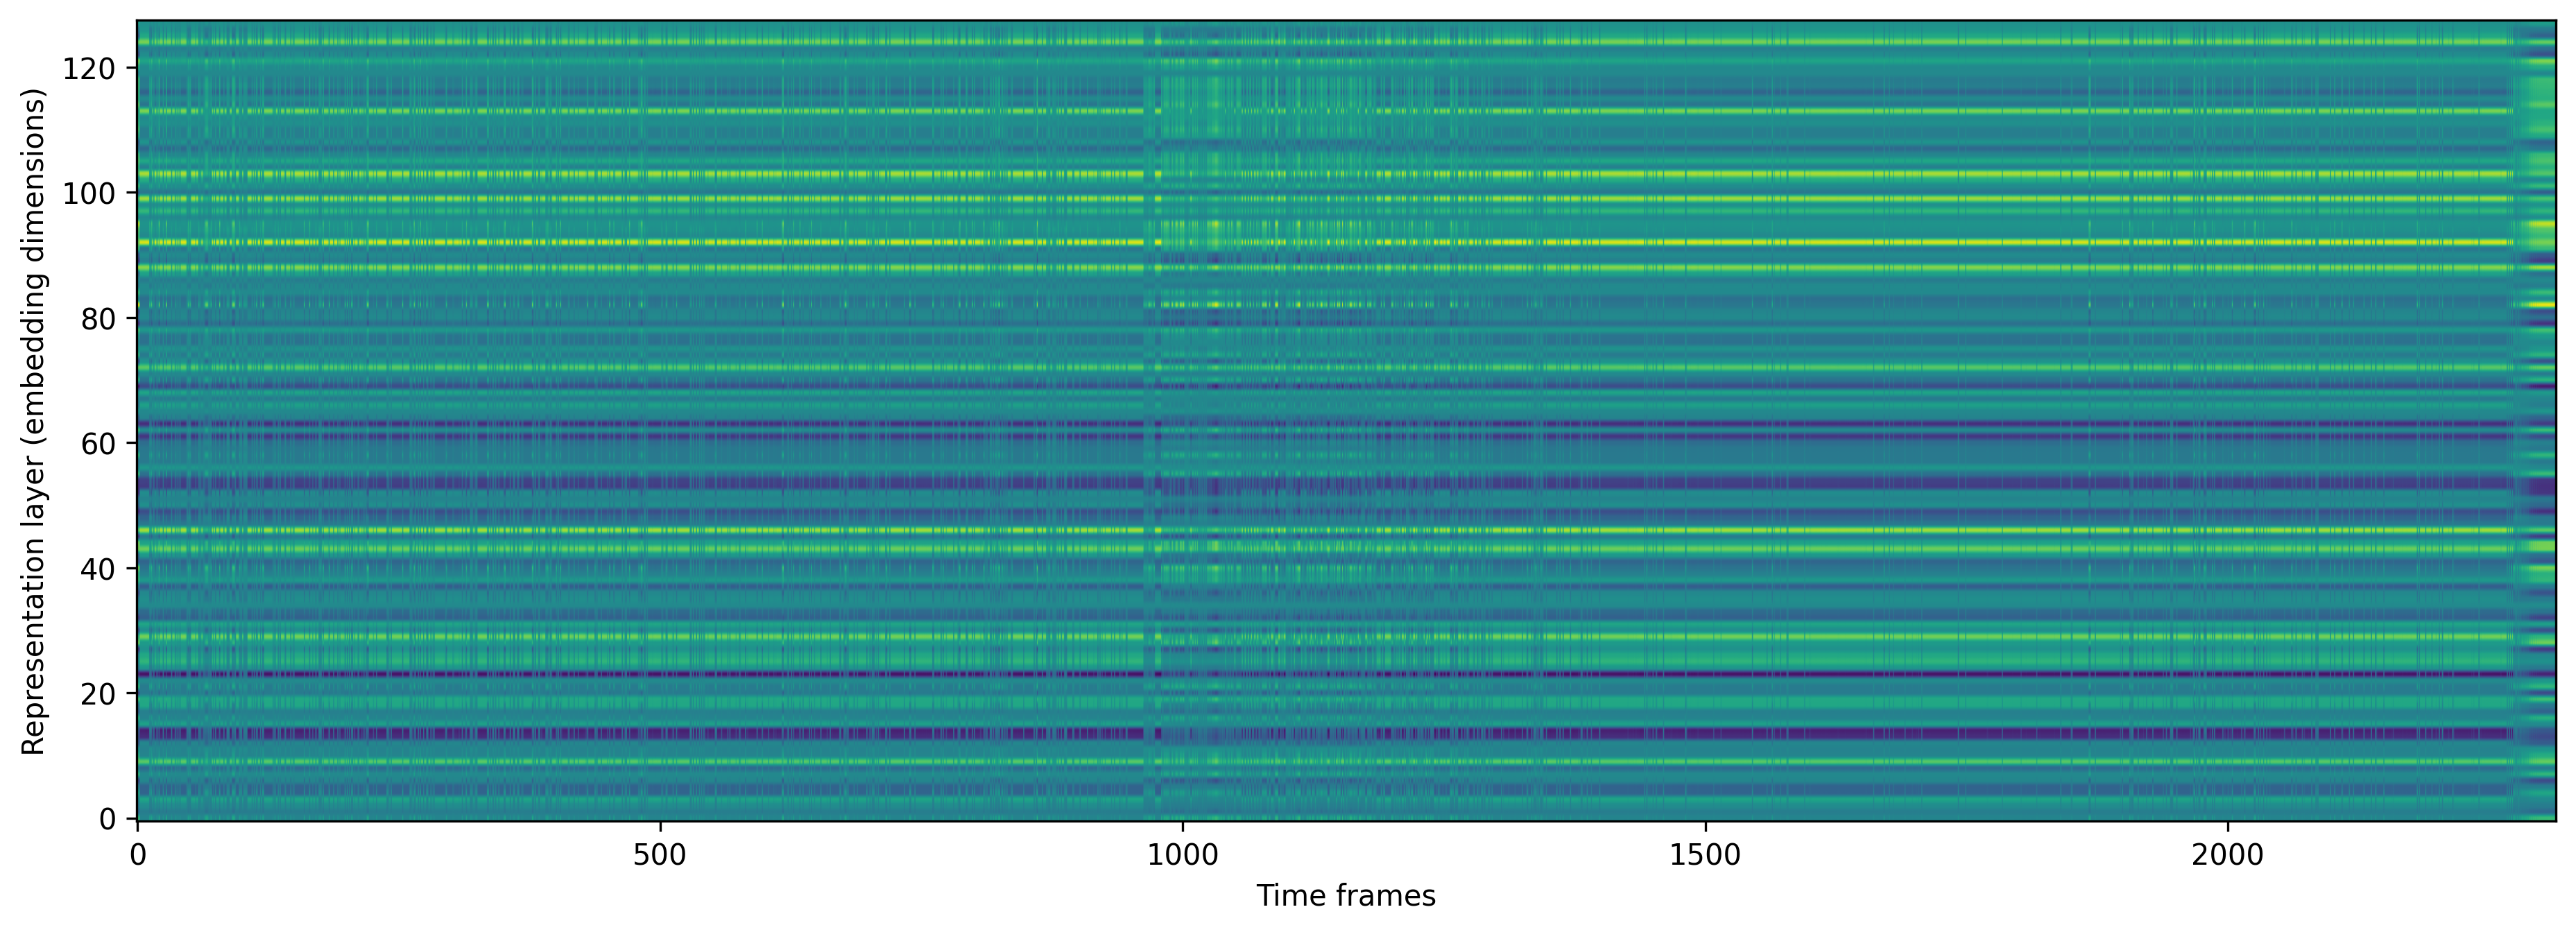
\includegraphics[width=\linewidth]{figures/images/salami_391_embeddiogram.png}
    \caption[]{Caption for image1}
    \label{fig:image1}
  \end{minipage}

  \begin{minipage}[b]{.8\linewidth}
    \centering
    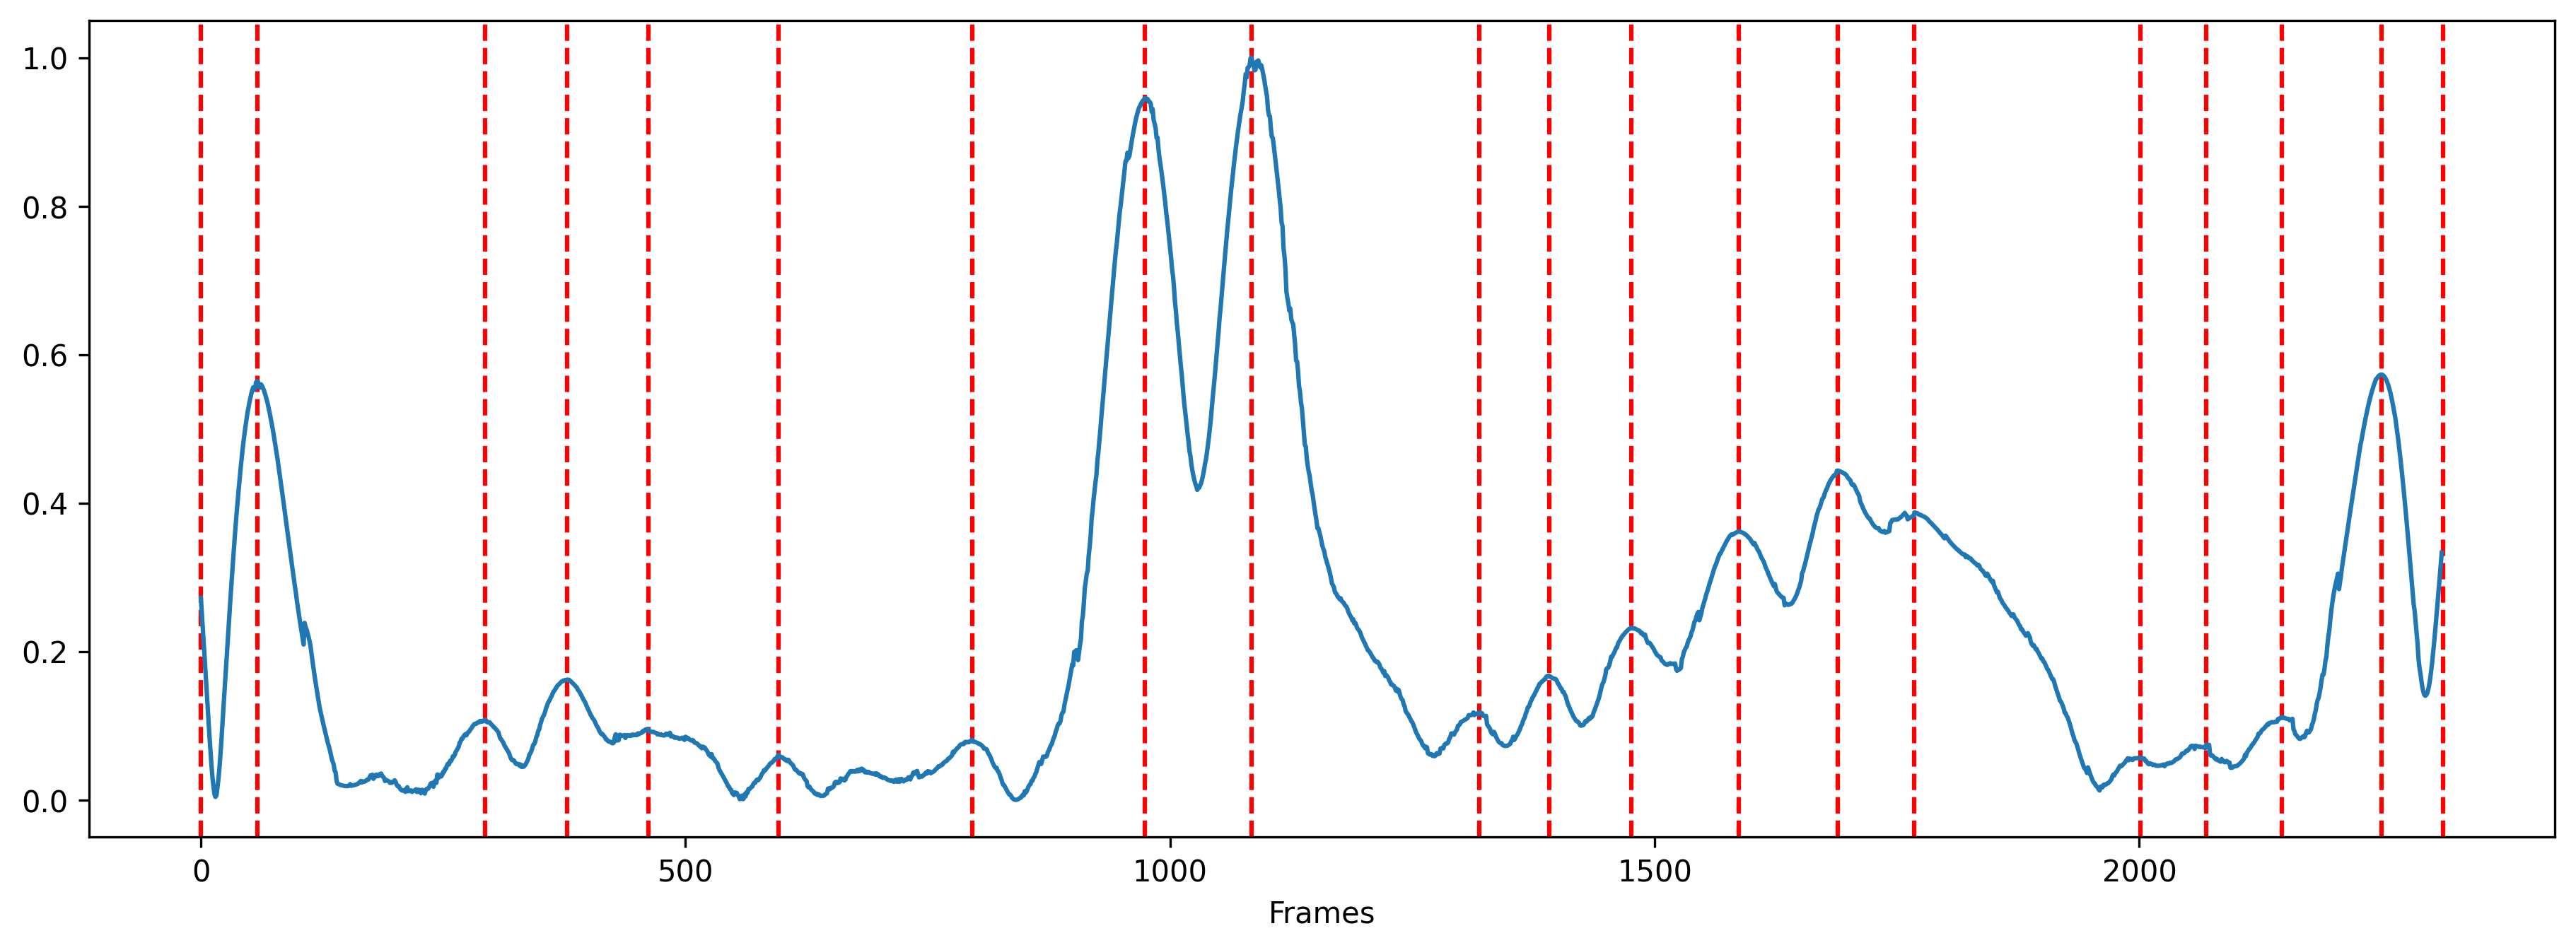
\includegraphics[width=\linewidth]{figures/images/samali_391_novelty_curve_peaks.png}
    \caption[]{Caption for image2}
    \label{fig:image2}
  \end{minipage}
\end{figure}


\begin{figure}[ht]
    \centering
    \begin{minipage}{0.45\textwidth}
        \centering
        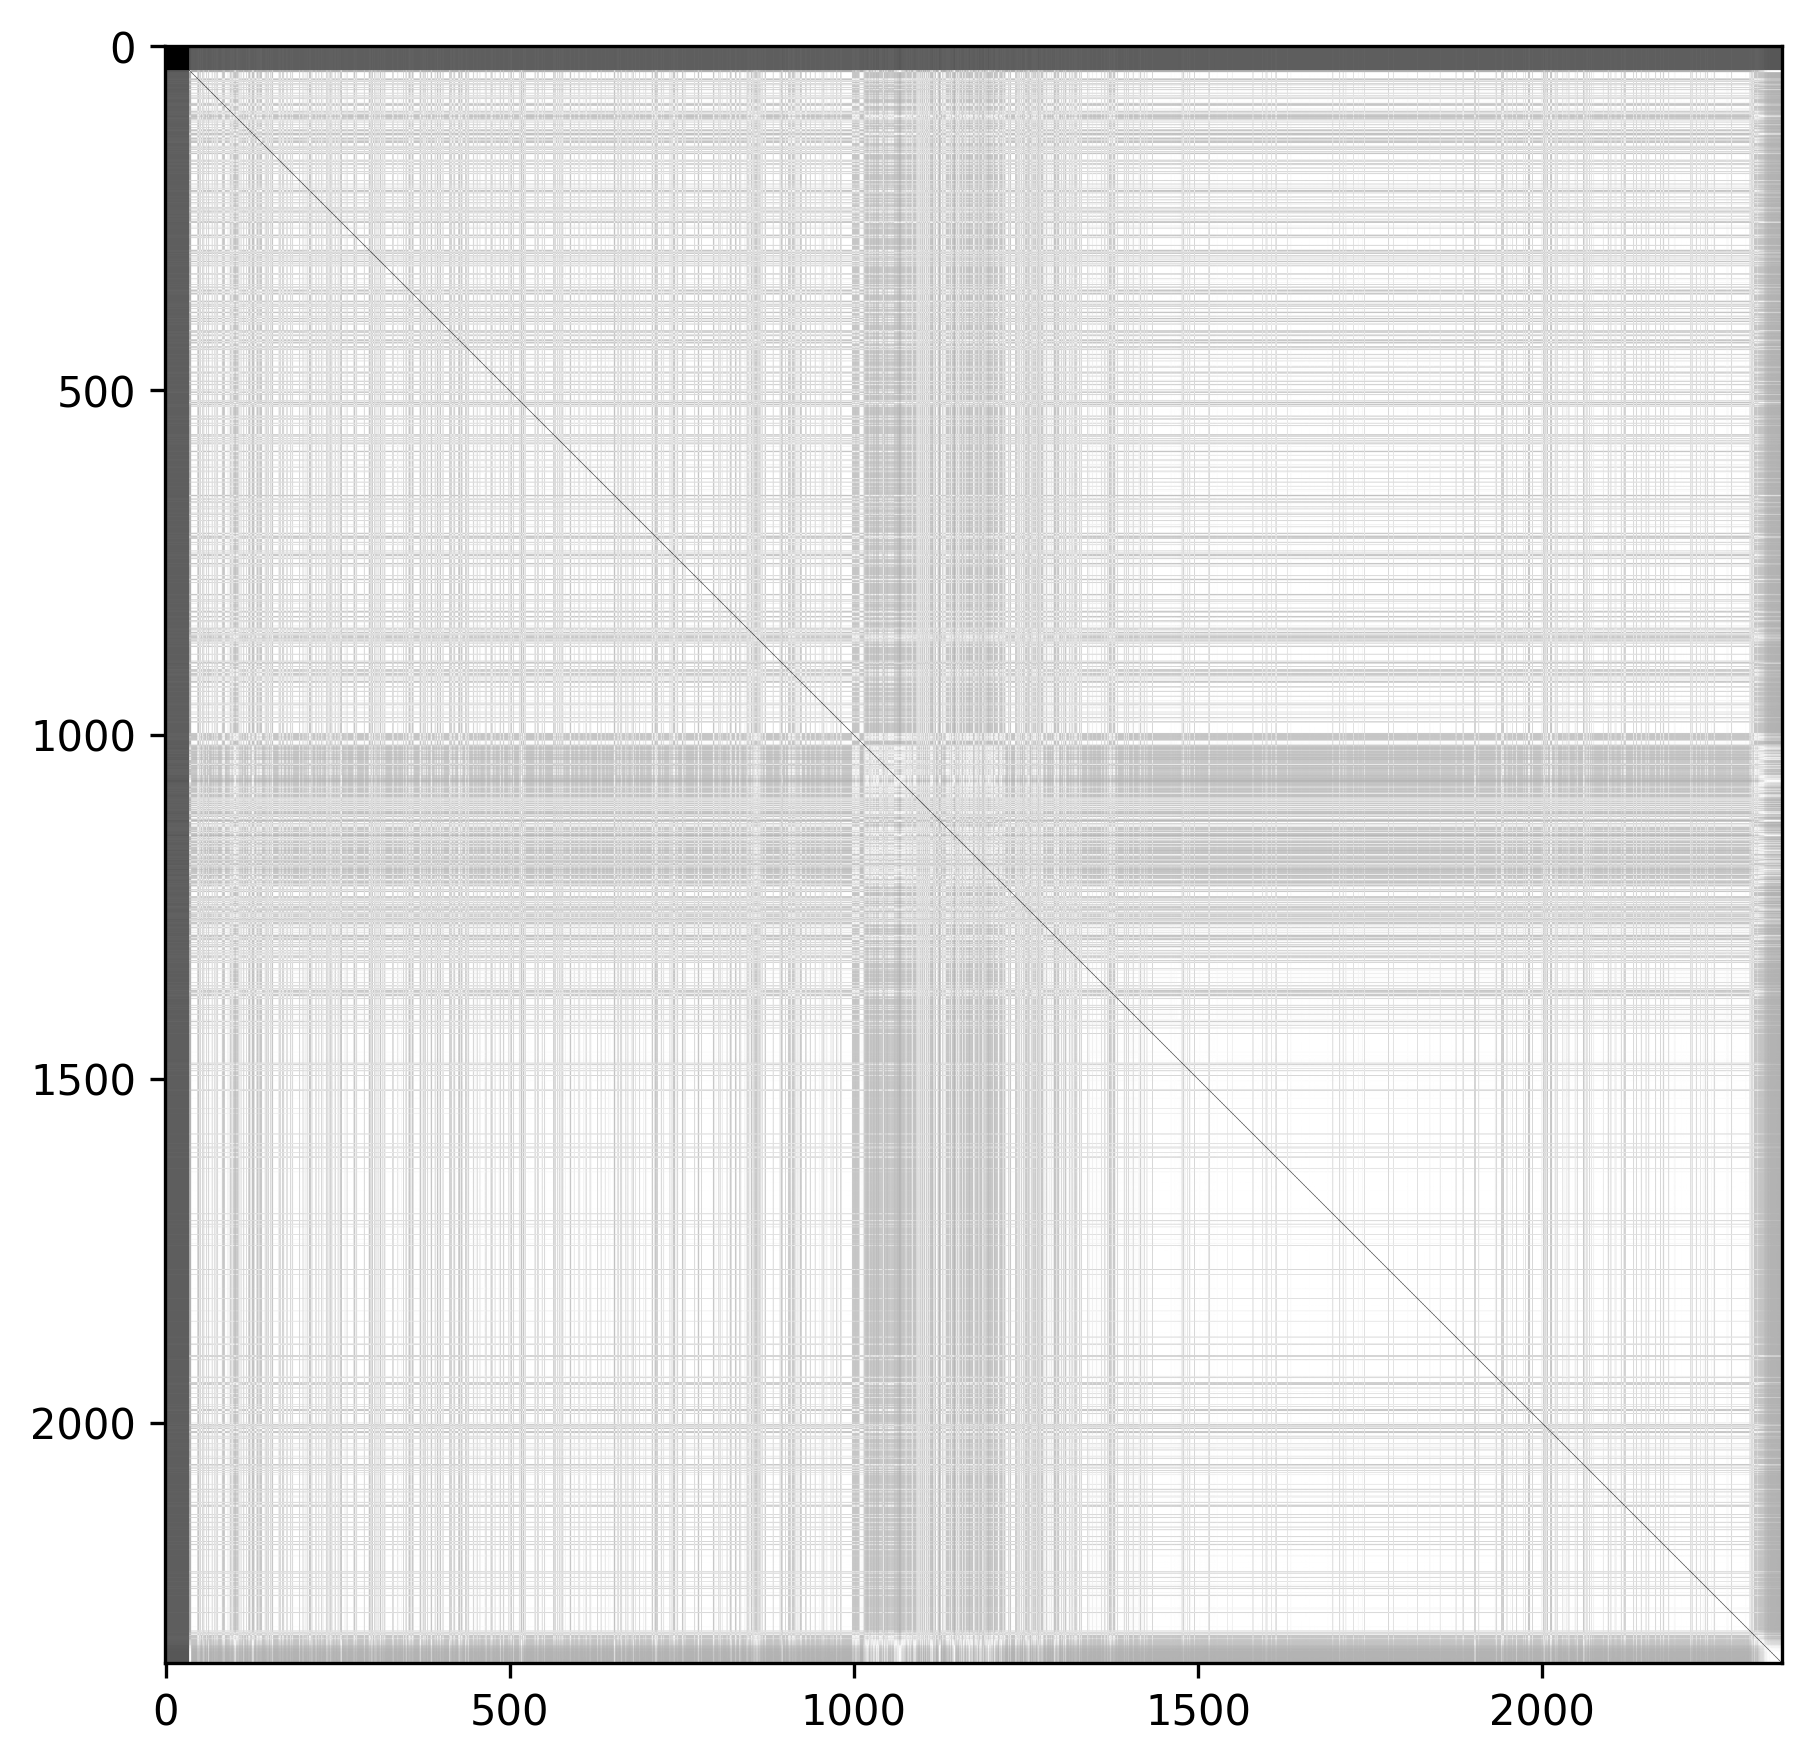
\includegraphics[width=0.9\textwidth]{figures/images/salami_391_R matrix after Gaussian smoothing.png} % first figure itself
        \caption[]{first figure}
    \end{minipage}\hfill
    \begin{minipage}{0.45\textwidth}
        \centering
        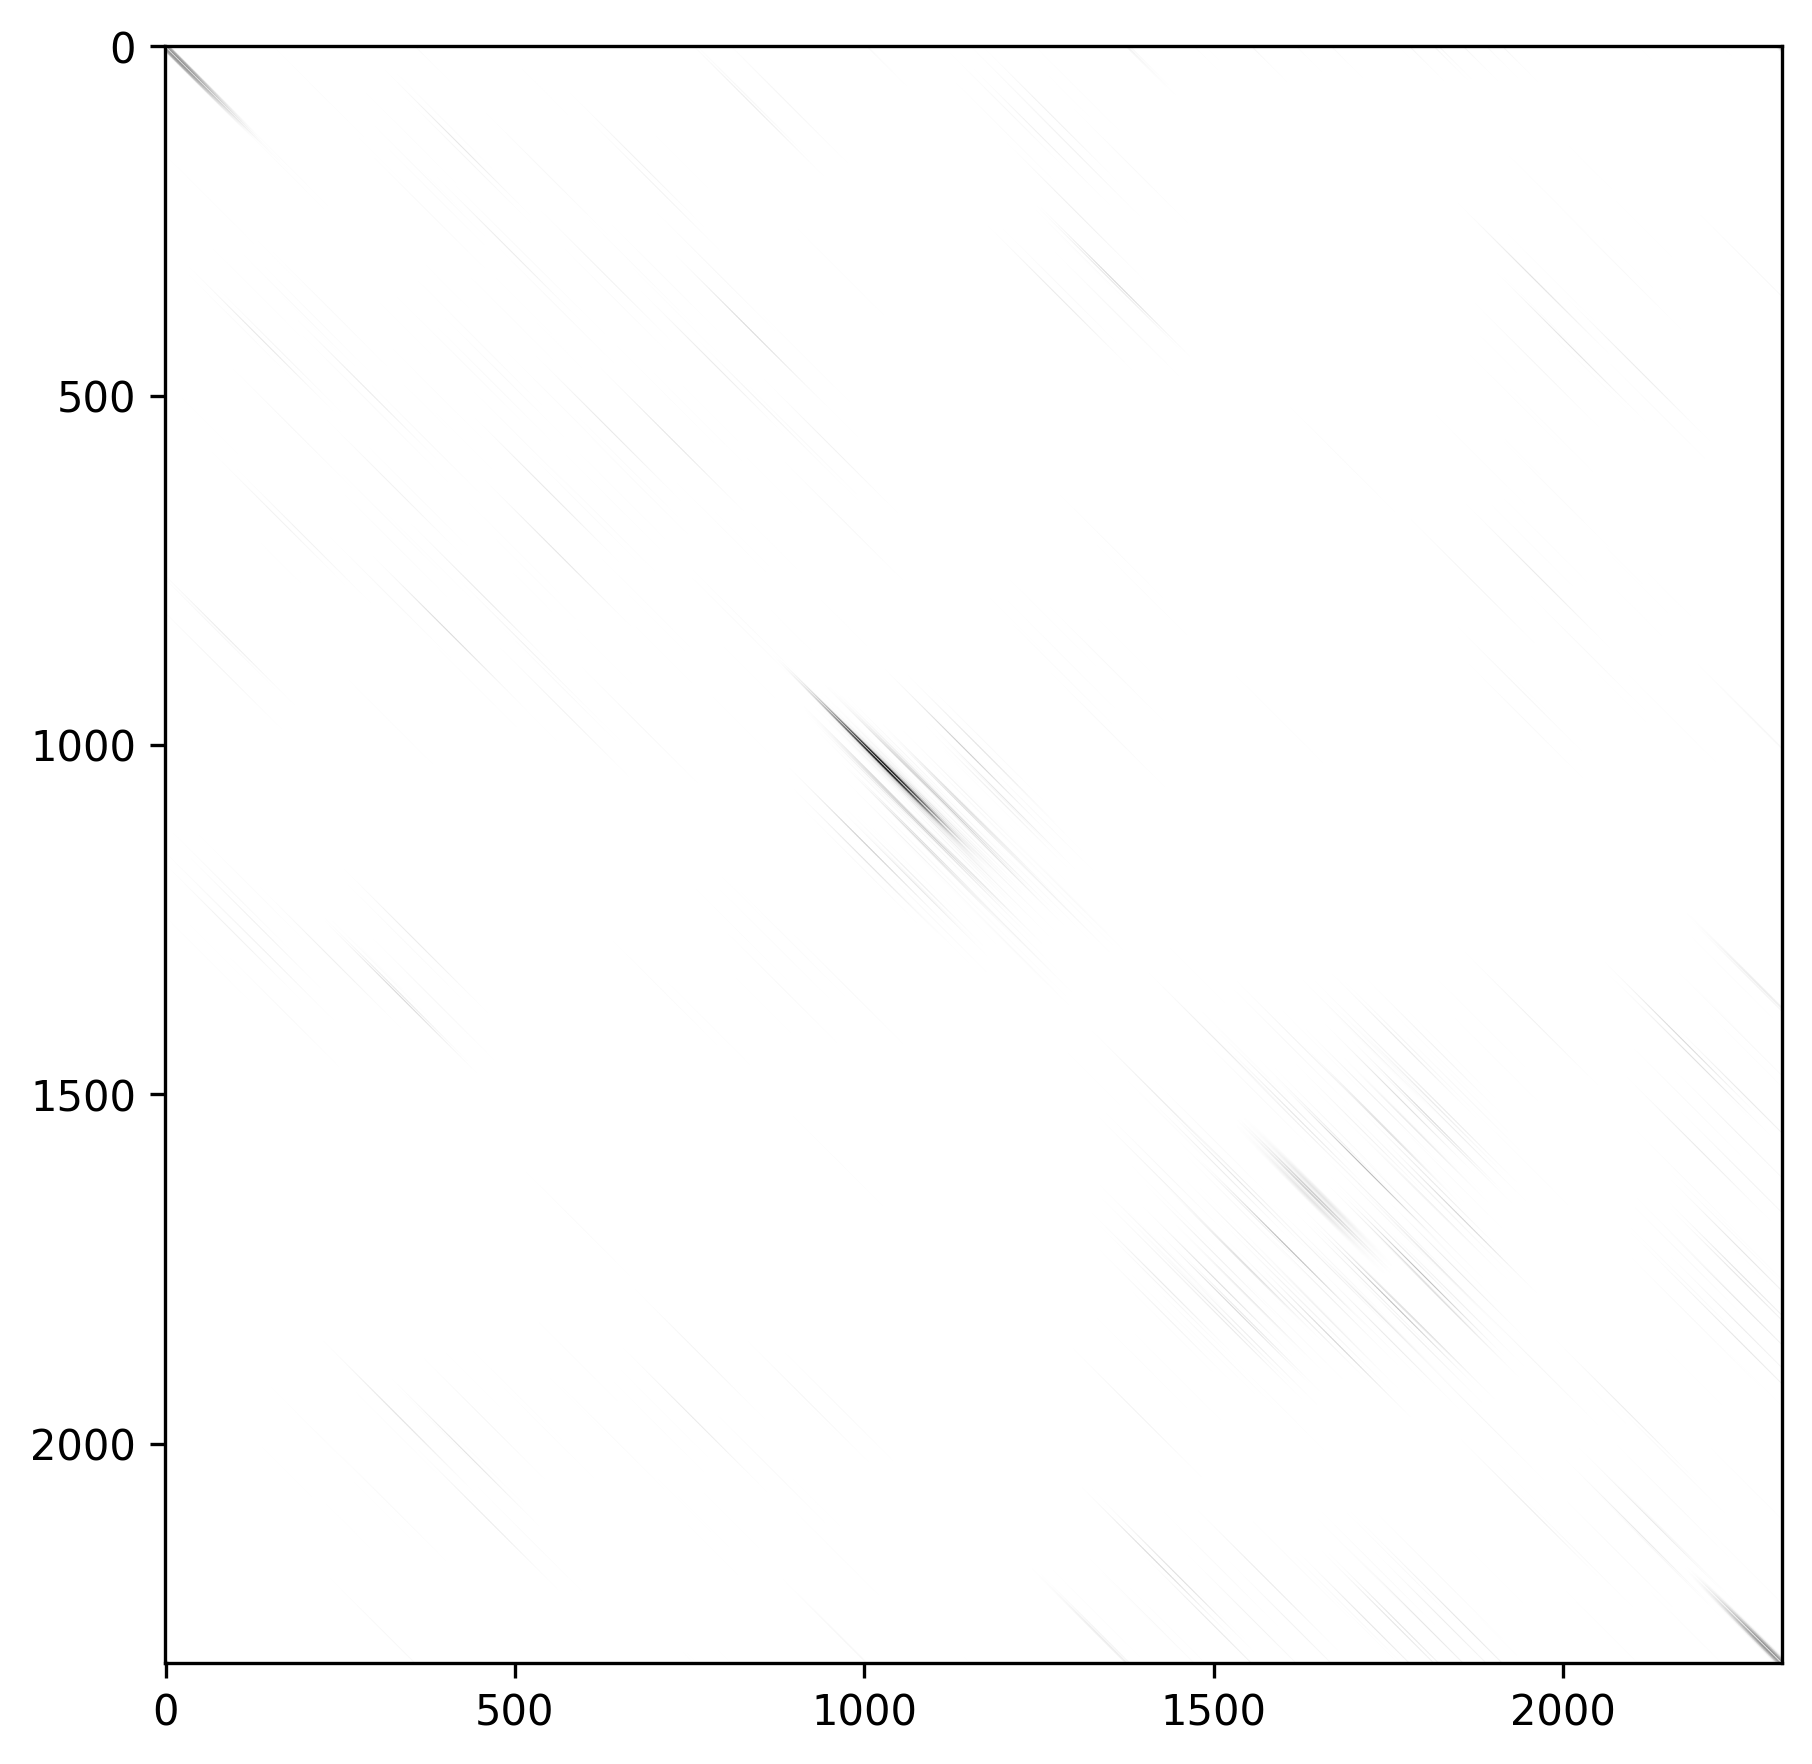
\includegraphics[width=0.9\textwidth]{figures/images/salami_391_Lag matrix after Gaussian smoothing.png} % second figure itself
        \caption[]{second figure}
    \end{minipage}
    \vfill
    \begin{minipage}{0.45\textwidth}
        \centering
        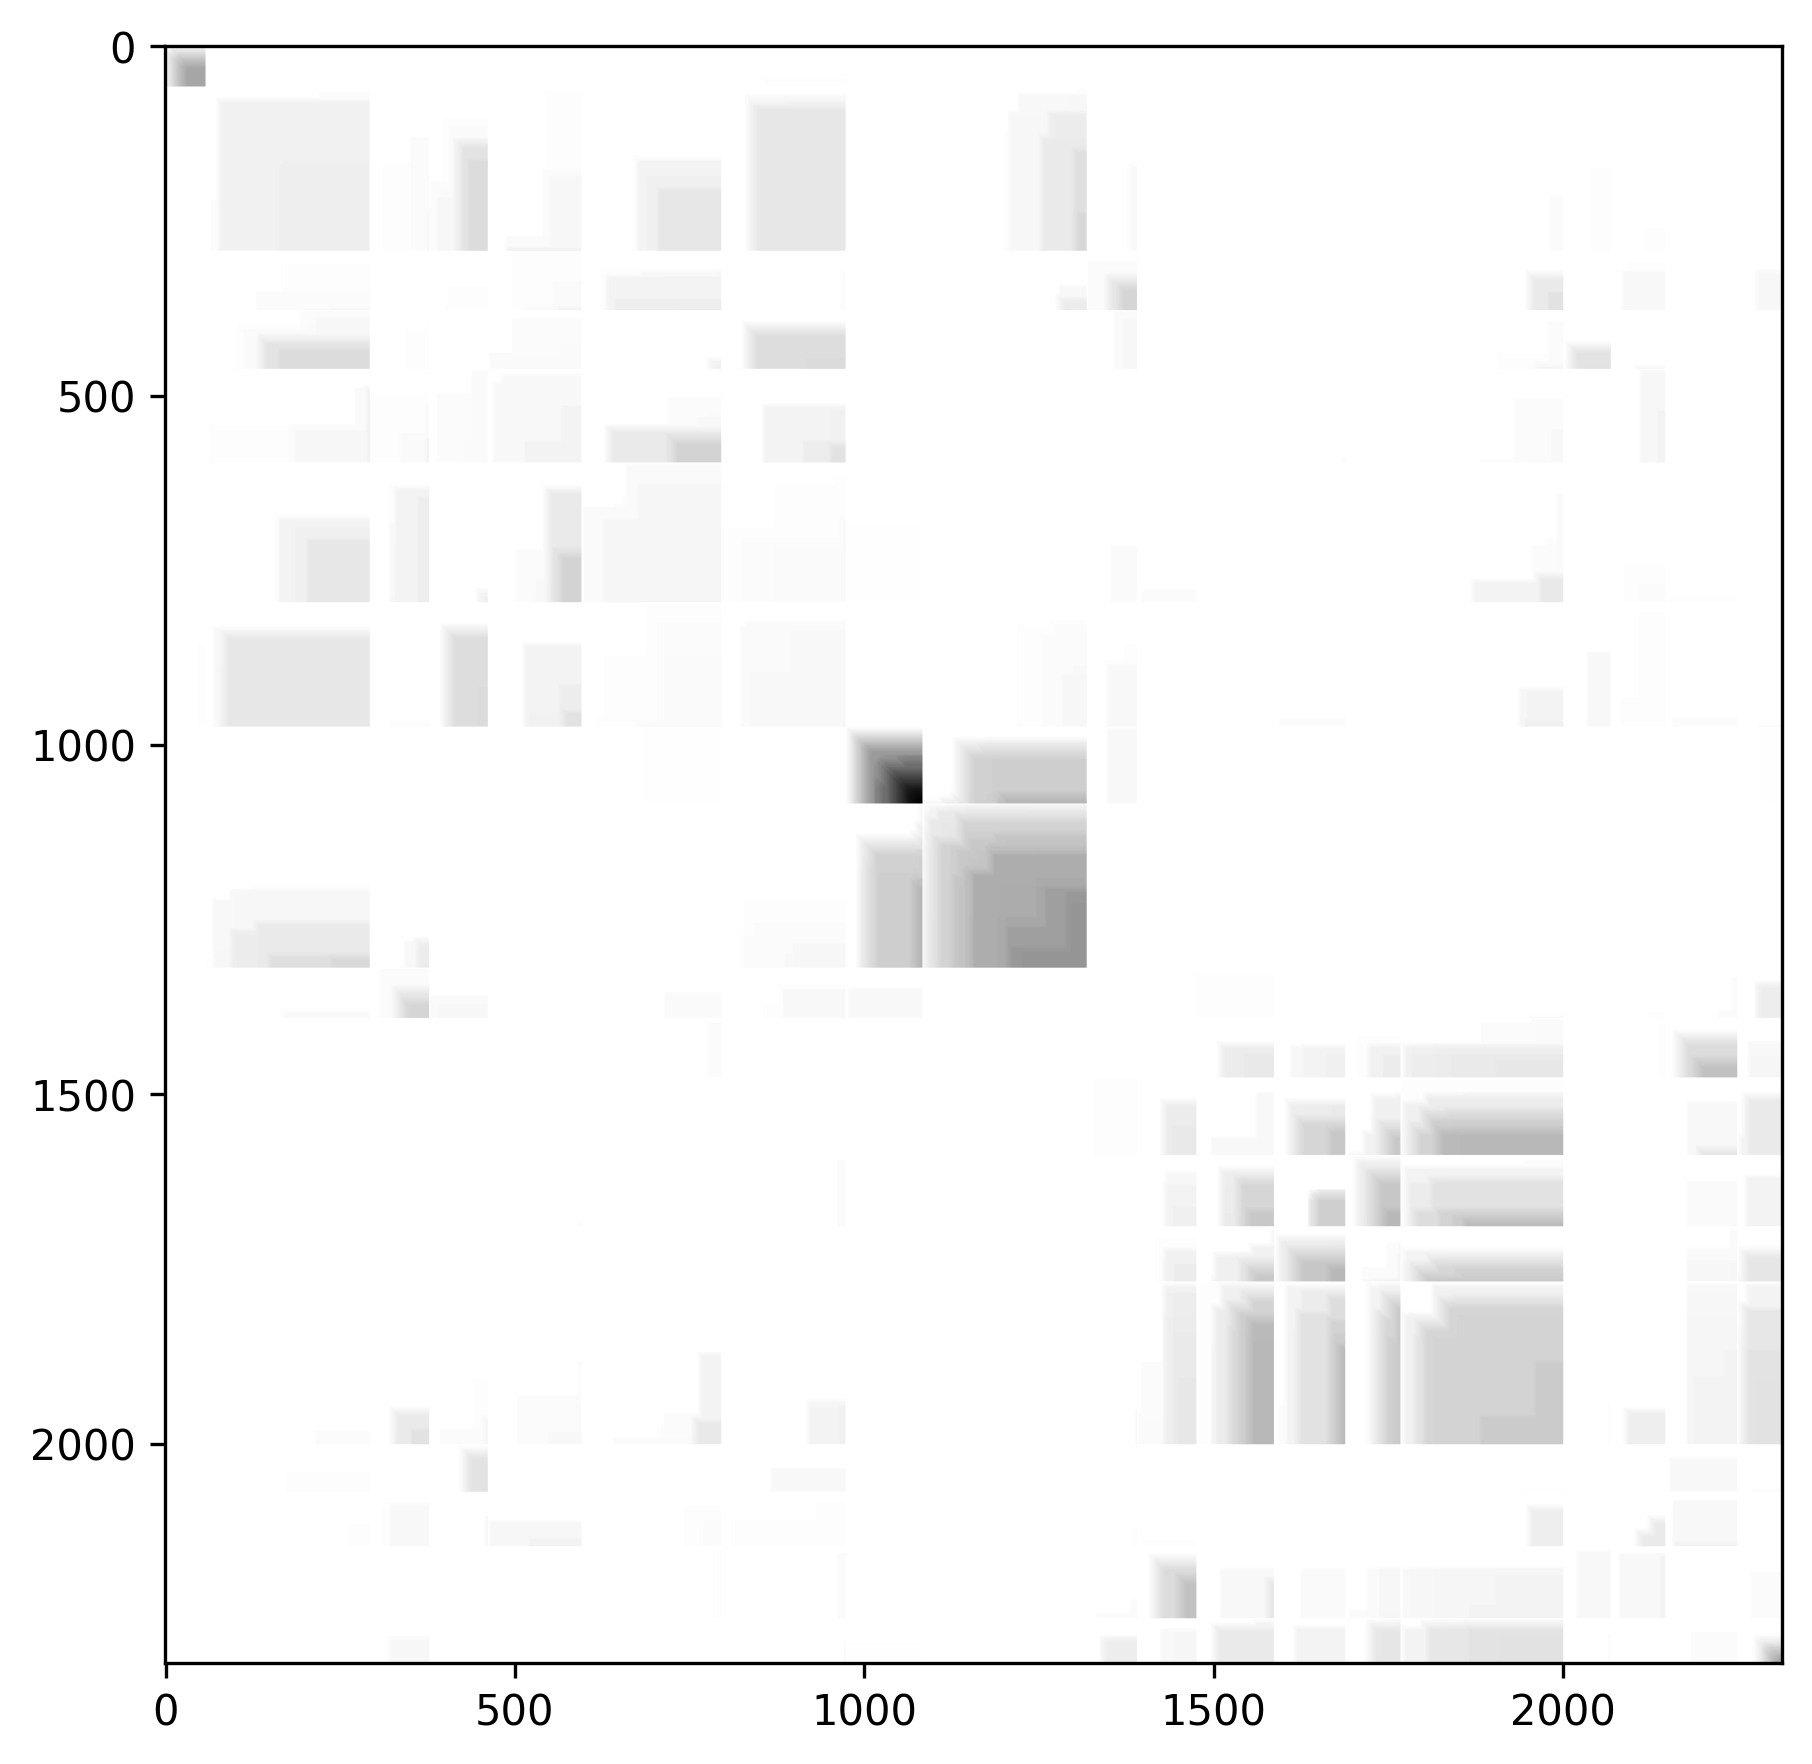
\includegraphics[width=0.9\textwidth]{figures/images/salami_391_Q_matrix.png} % third figure itself
        \caption[]{third figure}
    \end{minipage}\hfill
    \begin{minipage}{0.45\textwidth}
        \centering
        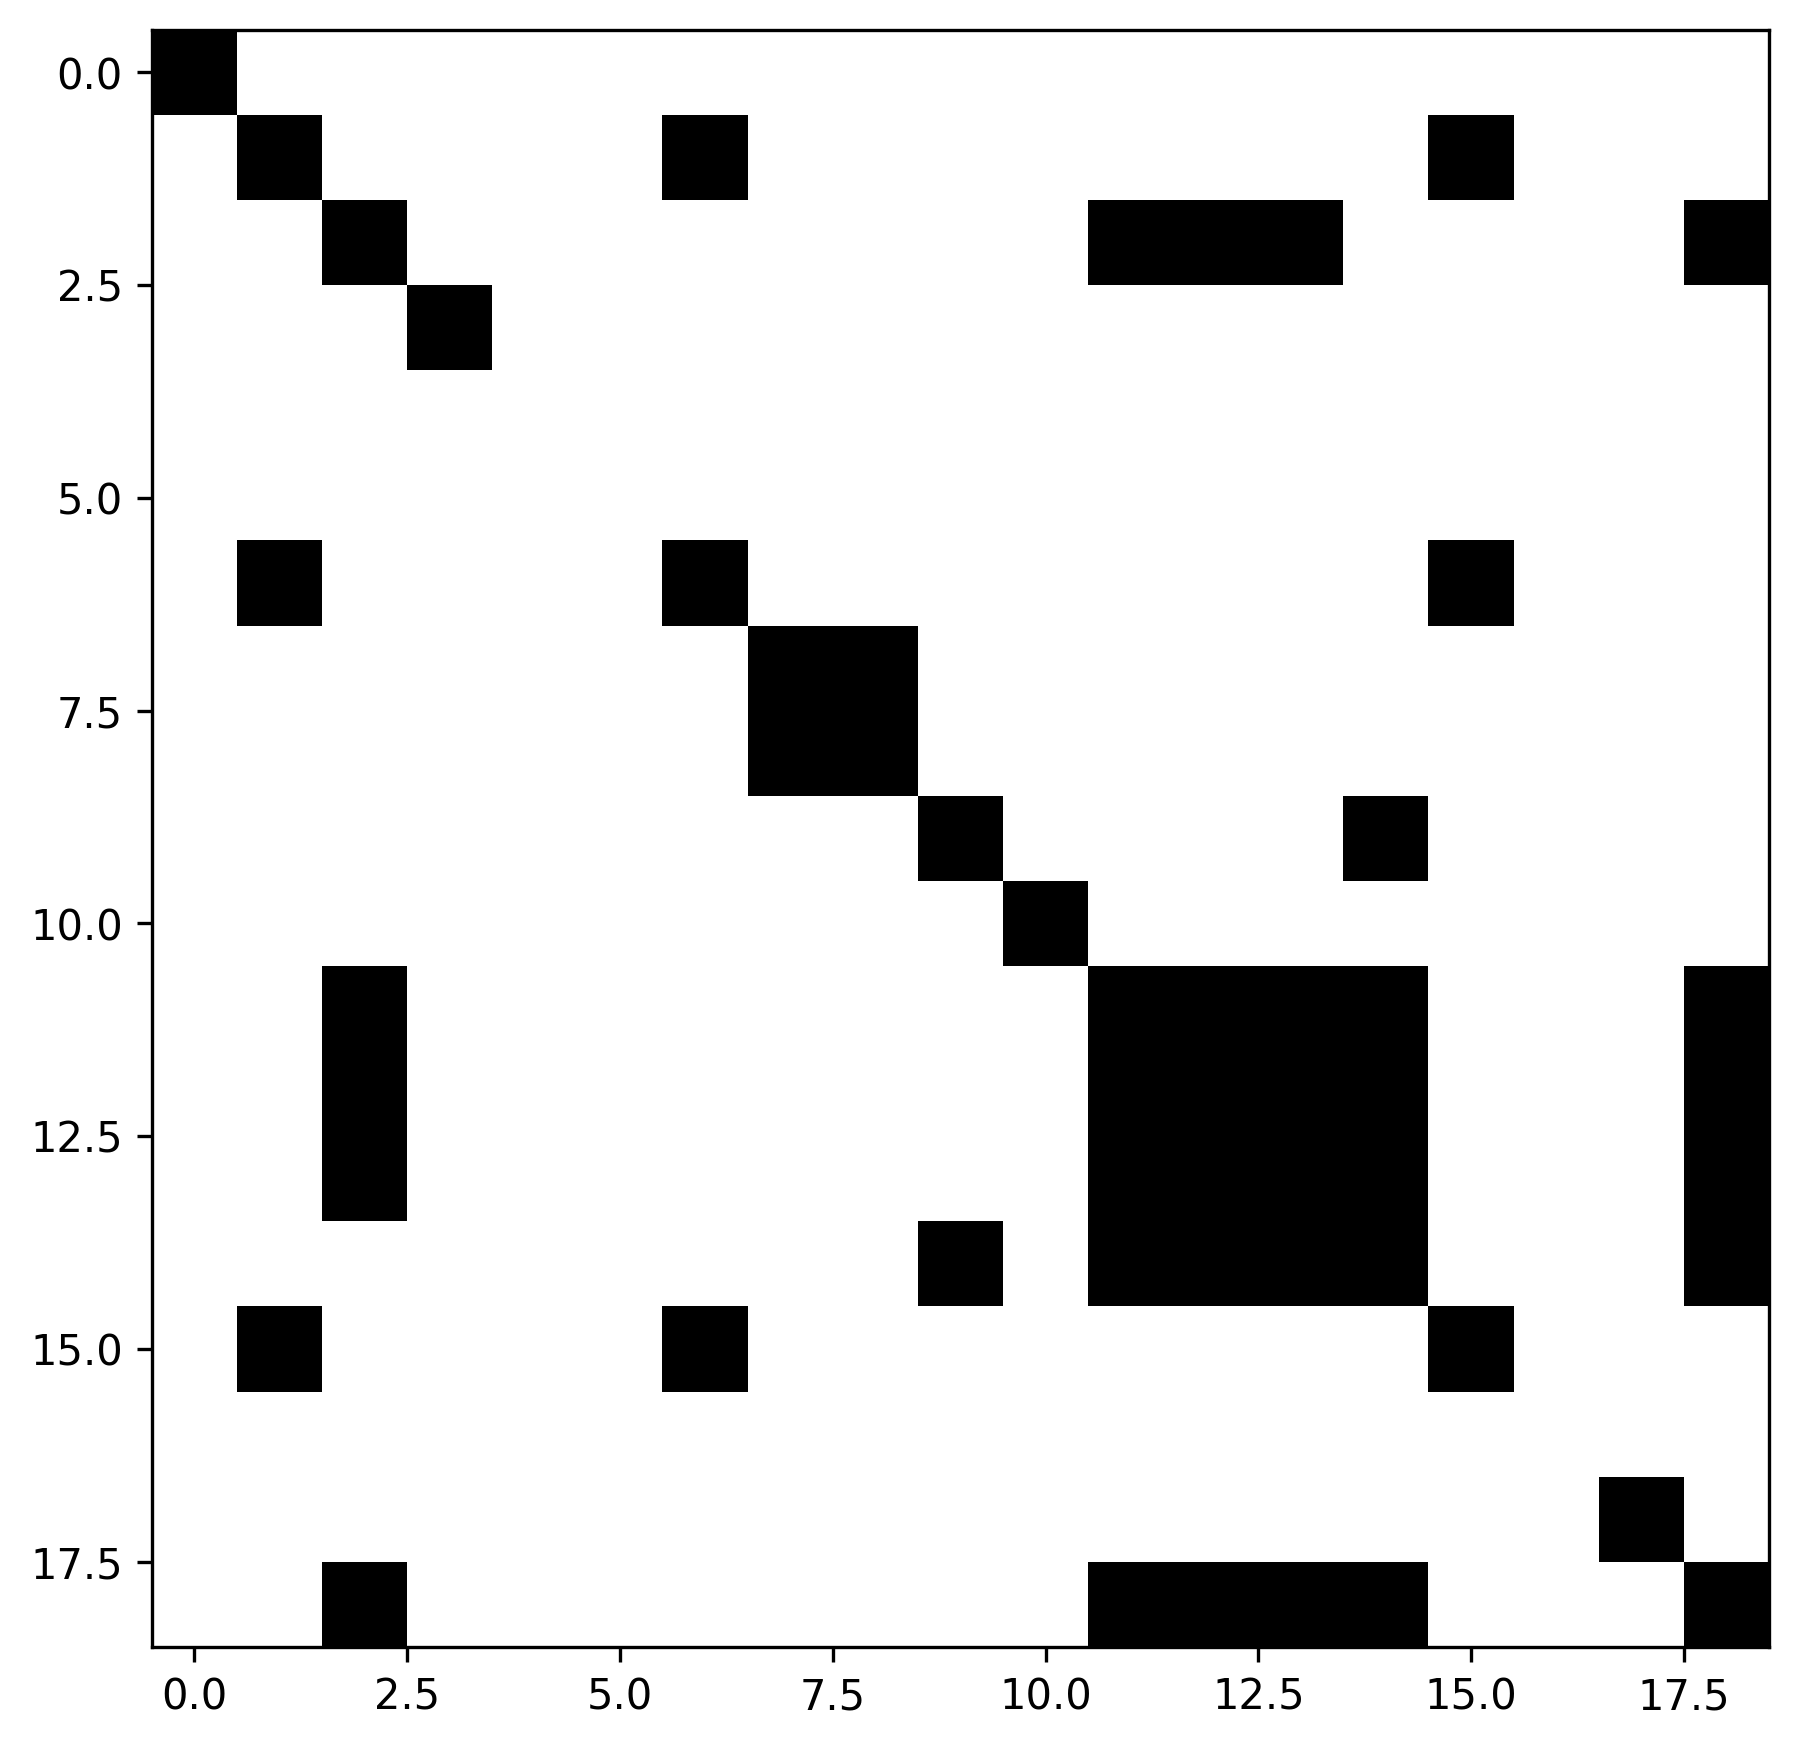
\includegraphics[width=0.9\textwidth]{figures/images/salami_391_binary transitive matrix.png} % fourth figure itself
        \caption[]{fourth figure}
    \end{minipage}
\end{figure}
